\documentclass[12pt,letterpaper,noanswers]{exam}
\usepackage[usenames,dvipsnames,svgnames,table]{xcolor}
\usepackage[margin=0.9in]{geometry}
\renewcommand{\familydefault}{\sfdefault}
\usepackage{multicol}
\pagestyle{head}
\header{AM 111 Class 14}{}{Approximating integrals, p.\thepage}
\runningheadrule
\headrule
\usepackage{siunitx}
\usepackage{graphicx} % more modern
\usepackage{amsmath} 
\usepackage{amssymb} 
\usepackage{hyperref}
\usepackage{tcolorbox}
\usepackage{enumitem}
\def\mbf{\mathbf}
\newcommand{\vc}[1]{\boldsymbol{#1}}
\def\dsst{\displaystyle}
\DeclareMathOperator*{\argmin}{arg\,min} % thin space, limits underneath in displays


\begin{document}
 \pdfpageheight 11in 
  \pdfpagewidth 8.5in

\noindent 

\section*{Preliminaries}

\begin{itemize}
\itemsep0pt
\item Problem set 06 is due by Friday at 5pm.  Submit extension requests in advance of that time.
\item There is a skill check in the next class.
\end{itemize}


\noindent\textbf{Big picture}

Today: Approximating $\int_{a}^{b}f(x)dx$.

\vspace{0.2cm}
\hrule
\vspace{0.2cm}

\noindent \textbf{Skill check practice}
\begin{questions}
\item Find the degree of precision of the following approximation for $\displaystyle\int_{-1}^1 f(x)dx$:
% $f(1)+f(-1)$, 
%$\dfrac{2}{3}[f(-1)+f(0)+f(1)]$, %$f\left(\dfrac{1}{\sqrt{3})\right) + f\left(\dfrac{1}{\sqrt{3})\right)$

$\displaystyle\int_{-1}^1 f(x)dx\approx 2f(0)$.

\emph{The following information may be helpful}
\[\int_{-1}^1 1\ dx = 2, \int_{-1}^1 x\ dx = 0, \int_{-1}^1 x^2\ dx = \frac{2}{3}, \int_{-1}^1 x^3\ dx =0, \int_{-1}^1 x^4\ dx = \frac{2}{5}\]
\item The skill from the Class 10 handout (Skill Check C11).
\end{questions}


\vspace{0.2cm}
\hrule
\vspace{0.2cm}

\noindent \textbf{Skill check solution}
\begin{questions}
\item For $f(x) = 1$, $2f(0) = 2$ so this is exact for $f$ constant.

For $f(x) = x$, $2f(0) = 0$ so this is exact for $f$ linear.

For $f(x) = x^2$, $2f(0) = 0$, which does not match.

The degree of precision is $1$.


\item See the past handout.
\end{questions}
\vspace{0.2cm}
\hrule
\vspace{0.2cm}

\noindent \textbf{Teams}
\begin{multicols}{3}
1. Mina, Basil, Johan

2. Nini, Brian, Eli

3. Nicolas, Aidan, Julia K

4. Mack, Benjamin, Robert

5. Alex, RJ, Jessica

6. Caitlin, Nina, Daniyal

7. Cameron, Dani, Emma

8. Eletria, Julia M, Tom

9. Ray, Ivonne, Shang

10.  Sophie, Eric, Alex

11. Jack, Esmé, Zachary

12. Kevin, Kevin, Marissa

\end{multicols}


\subsubsection*{Implementation}
\begin{enumerate}[resume=classQ]
\item Let \texttt{hvals} be an array of $h$ values (of length $N$) and \texttt{deriv} be the true value of $\frac{d}{dx}\sin x$ at $x = \pi/3$.
\begin{parts}
\item Write pseudocode for finding \texttt{error[k]}, the error associated with estimating $f'(x)$ for $h =$\texttt{hvals[k]}.
\vspace{1in}

%\item Write pseudocode for finding \texttt{extrapError[k]}, the error associated with estimating $f'(x)$ using extrapolation.  %It is your choice whether $h =$\texttt{hlist[k]} or $h/2 =$\texttt{hlist[k]}
\vspace{1in}

\item Write pseudocode for a loop that generates $N$ values of \texttt{error}.
\vspace{1.5in}

\item Vectorize your pseudocode.

Vectorized example:
\begin{multicols}{2}

\begin{verbatim}
# preliminaries
import numpy as np
f = np.sin
x0 = np.pi/3
h0 = 0.1
N = 52
\end{verbatim}
\columnbreak
\begin{verbatim}
# using a loop
hvals = np.zeros(N)
yvals = np.zeros(N)
for k in range(N):
    hvals[k] = h0
    yvals[k] = f(x0+h0)
    h0 = h0/2
\end{verbatim}

\end{multicols}
\begin{verbatim}
# vectorized
hvals = np.array([h0*2**(-k) for k in range(N)])
yvals = f(hvals+x0)
\end{verbatim}



% Add to your pseudocode in order to generate $N$ values of \texttt{extrapError}.  
\vspace{1in}
\end{parts}
\end{enumerate}
\section*{Numerical Integration}

Many integrals cannot be evaluated analytically.

\begin{tcolorbox}
\begin{itemize}
\itemsep0em
    \item The term \textbf{quadrature} is used to refer to finding an integral numerically.
    \item The name comes from \emph{quadratus} (square).  Early methods involved finding area under a curve by constructing a square of approximately the same area.
     \item For $\displaystyle\int_a^b f(x)dx$. a \textbf{quadrature rule} is determined by a set of nodes, $x_k \in [a,b]$, and a set of coefficients, $a_k$: $\displaystyle Q(f) = \sum\limits_{k=1}^n a_k f(x_k)$. 
     \item A quadrature rule for approximating an integral of a function $f$ has an associated \textbf{error}.  The error will depend on the properties of the function (specifically on its derivatives).
    \end{itemize}
    \end{tcolorbox}
    
\begin{tcolorbox}
\begin{itemize}
\itemsep0em    
   
    
    %The \textbf{left Riemann sum} for approximating an integral, $\displaystyle Q(f) = \sum\limits_{k=1}^n \frac{1}{n}f(a + (k-1)h)$ with $h = \frac{b-a}{n}$,  is an example of a quadrature rule.  The \textbf{right Riemann sum}, $\displaystyle Q(f) = \sum\limits_{k=1}^n \frac{1}{n}f(a + h)$ with $h = \frac{b-a}{n}$, is another example.
    
    \item \textbf{Composite} rules involve breaking the region of integration into subintervals and using an approximation method on each subinterval.  \emph{You may have seen this in your calculus class.}
\end{itemize}
\end{tcolorbox}

\subsection*{Newton-Cotes formulas}

(following Greenbaum and Chartier \S 10.1)

\begin{tcolorbox}
Approximate $\displaystyle\int_a^b f(x)dx$ by replacing $f$ with a polynomial interpolant.  Then integrate the polynomial.

For \textbf{Newton-Cotes} formulas, use equally spaced nodes to generate the interpolation.
\end{tcolorbox}
\begin{enumerate}[resume=classQ]
\item Assume $f(x) \in C^2[a,b]$.  $C^2$ means there is continuity of $f, f', f''$ on the interval.  

Use $x_0 = a, x_1 = b$ as the nodes for Lagrange interpolation, with $y_k = f(x_k)$.
\begin{parts}
    \item Write down $p_1(x)$, the first-degree polynomial interpolating $f$ at $x_0, x_1$.  
    \vspace{1cm}
    \item Find $\int_a^b p_1(x)dx$ as an approximation to $\int_a^b f(x)dx$.
    \vspace{1in}
    \item If you recognize this quadrature rule, what is it called?
    \vspace{0.5cm}
\end{parts}
\end{enumerate}

\begin{tcolorbox}
\begin{itemize}
\itemsep0pt
    \item Using a polynomial interpolant, $p(x)$, in place of $f(x)$, the \textbf{error} in the integral is given by $\displaystyle\int_a^bf(x)dx - \int_a^b p(x)dx.$
    \item For any point $x$ in $[a,b]$, $\displaystyle f(x) - p(x) = \frac{1}{(n+1)!}f^{(n+1)}(c_x)\prod\limits_{j=0}^n(x-x_j)$ for some point $c_x$ in $[a,b]$.
(see Greenbaum and Chartier \S 8.3, \S 8.4 for this error formula)
\end{itemize}
\end{tcolorbox}

\begin{enumerate}[resume=classQ]
\item We will find the error for the trapezoid rule.
\begin{parts}
\item
Use the formula above to write an integral expression for the error in the trapezoid rule.
\vspace{1cm}

\item What is the sign of $(x-a)(x-b)$ for $x\in [a,b]$?
\vspace{1cm}
\item Recall mean value theorem for integrals: Let $f:[a,b]\rightarrow\mathbb{R}$ be continuous, and $g$ an integrable function that does not change sign on $[a,b]$. Then there exists $c\in(a,b)$ such that $\displaystyle\int_a^b f(x)g(x) dx = f(c)\int_a^b g(x)dx$.

Use this theorem to remove $f''(c_x)$ from within the integral, and then evaluate the integral.

\emph{I suggest using integration by parts: Set $u = x-a, dv = (x-b)dx$.}
\vspace{1in}

\end{parts}
\end{enumerate}
You should find that the error is cubic in the size of the interval and proportional to the second derivative of $f$.
\begin{enumerate}[resume=classQ]
\item For any $f(x)$ linear in $x$, what will be the error for the trapezoid rule?
\vspace{1cm}
\end{enumerate}

\begin{tcolorbox}
\begin{itemize}
\itemsep0pt
    \item The {\bf degree of precision} of a numerical integration method is the greatest integer $k$ for which all polynomials of degree $k$ or less are integrated exactly by the method.
\item The trapezoid rule has a degree of precision of $1$.
\end{itemize}

\end{tcolorbox}
%\noindent\textbf{Simpson's rule}
\begin{tcolorbox}
\textbf{Simpson's rule} is generated by using quadratic interpolation on $f$ at with interpolation points $x_0 = a, x_1 = \frac{a+b}{2}, x_2 = b$.
\end{tcolorbox}
\begin{enumerate}[resume=classQ]
    \item Let $p_2(x) = y_0L_1(x) + y_1L_2(x)+y_2L_3(x)$ where $x_0 = a, x_1 = (a+b)/2, x_2 = b$ and $y_k = f(x_k)$.  
    
    $\displaystyle\int_a^b p_2(x) = A_0 y_0 + A_1 y_1 + A_2 y_2$.  You can find $A_0, A_1, A_2$ by integrating $L_1, L_2, L_3$.  Instead of integrating, use the integral information in the caption of the figure below to find $A_0, A_1, A_2$.  Note that $h = (b-a)/2$.
\end{enumerate}


    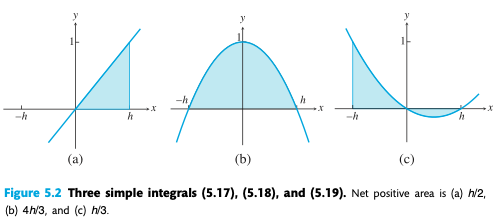
\includegraphics{img/Class12Sauerintegrals.png}
\begin{enumerate}[resume=classQ]
    \item The \textbf{method of undetermined coefficients} is another option for finding $A_0, A_1, A_2$.
    \begin{parts}
    \item For $f(x)$ a constant, linear, or quadratic polynomial, $\int_a^b f(x)dx = A_0 y_0 + A_1 y_1 + A_2 y_2$ is exact.
    
    Let $f(x) = 1$.  Use $\int_a^b 1\ dx = A_0  + A_1 + A_2 $ to find an equation for $A_0+A_1+A_2$ in terms of $a$ and $b$.
    \vspace{1in}
    \item Repeat this for $f(x) = x$ and $f(x) = x^2$ to generate two more equations in terms of $A_0, A_1, A_2$ and $a,b$.
    \vspace{2in}
    \item Write your linear system as a matrix equation.
    \vfill
    \end{parts}
    
The solution to the system is $A_0 = A_2 = \dfrac{b-a}{6}$, $A_1 = 4\dfrac{b-a}{6}$.
\end{enumerate}
\begin{tcolorbox}
\noindent\textbf{Simpson's rule}

Given a function $f(x) \in C^4[a,b]$, let $h = \dfrac{b-a}{2}$.
\[
          \int_{a}^{b} f(x) \, dx = \frac{h}{3}\left[ f(a)+4f\left(\dfrac{a+b}{2}\right) + f(b) \right]
          - \frac{h^5f^{(iv)}(c)}{90}.\]
\end{tcolorbox}



\begin{enumerate}[resume=classQ]
    \item Show that the degree of precision for Simpson's rule is $3$.
    
    To do this, we need to show that $\int_a^b 1\ dx$, $\int_a^b x\ dx$, $\int_a^b x^2\ dx$, $\int_a^b x^3\ dx$ are all integrated exactly by Simpson's rule.

$\int_a^b 1\ dx$, $\int_a^b x\ dx$, $\int_a^b x^2\ dx$ are integrated exactly by construction of the rule, so what is left to show is that $\int_a^b x^3\ dx$ is integrated exactly.
    \begin{parts}
    \item One way to do this is to shift your integral.  Find $k$ such that $\int_a^b x^3 dx = \int_{-h}^h (x+k)^3 dx$.
    \vspace{1cm}
    
    \item Expanding, $(x+k)^3 = x^3 + q(x)$ where $q(x)$ is a quadratic function.  
    
    $\int_a^b x^3 dx = \int_{-h}^h (x+k)^3 dx = \int_{-h}^h x^3 dx  + \int_{-h}^h q(x) dx$
    
    Provide an argument for why each term of the final expression is zero.
    \vspace{1.5in}
    
    
    
    \end{parts}
    
\end{enumerate}

\subsection*{Composite rules}
\begin{tcolorbox}
(from Sauer \S 5.2.3)
\begin{itemize}
\itemsep0pt
    \item For a composite rule, approximate $\displaystyle\int_a^b f(x)dx$ by breaking $[a,b]$ into adjacent subintervals, or \textbf{panels}.
    \item The \textbf{composite Trapezoid rule} is the sum of the Trapezoid rule applied to each panel.
    \item For a function $f\in C^2[a,b]$, choose an evenly spaced grid: $a = x_0<x_1<...<x_{m-1}<x_m = b$ with $h = x_k-x_{k-1} = (b-a)/m$.  \[\displaystyle\int_a^b f(x)dx = \frac{h}{2}\left(y_0 + \sum\limits_{k=2}^{m-1}y_k + y_m \right) - (b-a)\frac{h^2}{12}f''(c),\] where $c$ is between $a$ and $b$.
\end{itemize}
\end{tcolorbox}
\begin{enumerate}[resume=classQ]
    \item In a single panel, the error from the Trapezoid rule is given by $-\frac{1}{12}h^3f''(c_k)$ with $x_{k-1}<c_k<x_k$.
    \begin{parts}
    \item Find an expression for the sum of the error over all $m$ panels (use summation notation).
    
\vspace{1in}
\item The generalized intermediate value theorem says that for $f$ continuous on $[a,b]$, $c_k$ points in $[a,b]$, and weights $w_1, ..., w_m>0$, there exists a number $c$ between $a$ and $b$ such that $w_1f(c_1)+...+w_mf(c_m) = (w_1+...+w_m)f(c)$.  Use this theorem to write your expression as $f''(c)$ times a constant.  Write the constant in terms of $m$ and $h$.
\vspace{1in}
\item Is the error you found equal to $- (b-a)\frac{h^2}{12}f''(c)$?
\vspace{1cm}
    \end{parts}
\end{enumerate}

The error in the Trapezoid rule is proportional to $f''$ and to $h^3$.

The error in the composite Trapezoid rule is proportional to $f''$ and to $h^2$.

\begin{enumerate}[resume=classQ]
\item For composite Simpson's rule, let each panel be length $2h$.  Use the grid $a = x_0 < x_1 < ... < x_{2m-1}<x_{2m}$.
\begin{parts}
\item For $a = x_0, b = x_2$, Simpson's rule can be written $\int_a^b f(x)dx \approx \frac{h}{3}(y_0 + 4y_1 + y_2)$.

The composite rule is of the form \[\frac{h}{3}\left[y_0 + A \sum\limits_{k=1}^m y_{2k-1} + B\sum\limits_{k=1}^{m-1}y_{2k} + y_{2m}\right].\]

Find $A$ and $B$.
\end{parts}
\end{enumerate}

\subsection*{Open vs closed formulas}
\begin{tcolorbox}
\textbf{Closed} Newton-Cotes formulas use $f(a)$ and $f(b)$ in the approximation.

\textbf{Open} Newton-Cotes formulas avoid values from the ends of the intervals.
\end{tcolorbox}
\begin{enumerate}[resume=classQ]
    \item To approximate $\displaystyle\int_a^b f(x)dx$, let $x_0 = a, x_1 = b$, $h = b-a$.  Set $w = x_0 + h/2$ (the midpoint of the interval).
    \begin{parts}
    \item Find the degree $1$ Taylor expansion of $f(x)$ about the midpoint $w$.  Do this exactly, so include the remainder term (it is $\frac{1}{2}(x-w)^2f''(c_x)$.
    \vspace{1in}
    \item Integrate both sides from $a$ to $b$.
    
    Note that $f'(w)$ is a constant.  Use the mean value theorem for integrals to remove $f''(c_x)$ from the integral.
    \vspace{1in}
    
    \end{parts}
This generates the \textbf{midpoint rule} for approximating an integral.
\end{enumerate}
\begin{tcolorbox}
The \textbf{composite midpoint rule} is given by \[\int_a^bf(x)dx = h\sum\limits_{i=1}^m f(w_i) + \frac{1}{24}(b-a)h^2 f''(c)\] where $h = (b-a)/m$ and $a<c<b$.  The $w_i$ are midpoints of the $m$ equal subintervals of $[a,b]$.
\end{tcolorbox}
% \fbox{
%     \begin{minipage}{15cm}
%       \subsection*{Midpoint Rule}
%       Given a function $f(x) \in C^2(x_0,x_1)$ and points $x_0<x_1$, $x_1-x_0 = h$,
%             \begin{equation}
%           \int_{x_0}^{x_1} f(x) \, dx = h(f(x_0+ h/2)) + \frac{h^3}{24} f''(c)
%         \end{equation}
%     \end{minipage}}

% \vspace{10cm}


%     \fbox{
%     \begin{minipage}{15cm}
%       \subsection*{Composite Midpoint Rule}
%       Given a function $f(x) \in C^4(a,b)$ and equally spaced
%       points $a=x_0<x_1<\cdots<x_{2m}=b$, $x_{i+1}-x_i = h$,
%       \begin{equation}
%         \int_a^b f(x) \, dx = h \sum_{i=1}^m f\left(\frac{x_{i-1} + x_i}{2}\right) + \frac{(b-a)h^2f''(\xi)}{24}.
%       \end{equation}
%     \end{minipage}}

% \pagebreak

% \subsection*{Adaptive Quadrature}

% \pagebreak

% \been

% \item Read the adaptive quadrature algorithm in the book (\S5.4) and implement it to estimate:

% \beit
% \item $\int_{-1}^1   2\sqrt{1-x^2} dx$
% \item $\int_{-1}^1   1+\sin(e^{3x}) dx$
% \enit

% \enen



%
%\subsection*{Romberg Integration}
%
%\been
%
%\item[4.] Romberg integration uses the composite trapezoid rule with successively
%smaller stepsizes $h$.
%
%\been
%\item {\bf Romberg Integration (First Column)}
%
%Define stepsizes $h_j$ such that each successive stepsize is half the
%previous stepsize:
%\begin{align*}
%h_1 &= b-a \\
%h_2 &= (b-a)/2 \\ 
%h_3 &= (b-a)/4 \\
%& \vdots \\
%h_j&=\frac{1}{2^{j-1}}(b-a).
%\end{align*}
%
%The first column of Romberg integration, $R_{j1}$, is the composite
%trapezoid rule applied to the function on $[a,b]$ with stepsize $h_j$.  Write down the formula for the first few elements of the first column:
%
%\vfill
%
%\begin{align*}
%R_{11} &= \blank{3in} \\
%& \\
%R_{21} &= \blank{3in} \\
%& \\
%R_{31} &= \blank{3in}
%\end{align*}

%\pagebreak
%
%The second column applies Richardson extrapolation to the 1st column
%$R_{j1}$.  Write down the results for the second column.  What is $R_{22}$?
%
%\vfill
%
%\begin{align*}
%R_{22} &= \frac{2^2 R_{21} - R_{11}}{3} = \blank{3in} \\
%& \\
%R_{32} &= \frac{2^2 R_{31} - R_{21}}{3} = \blank{3in}
%\end{align*}
%
%\item Calculate $R_{11}$, $R_{21}$, and $R_{22}$ for $\dsst{\int_0^4 x^2 \, dx}$.
%
%\vfill
%
%\pagebreak
%
%\item The third column applies Richardson extrapolation to the second column.
%Because the second column is composite Simpson's rule, it is 4th order in $h$:
%\begin{align*}
%R_{33} &= \frac{4^2 R_{32} - R_{22}}{4^2-1} \\
%R_{43} &= \frac{4^2 R_{42} - R_{32}}{4^2-1} \\
%& \vdots \\
%R_{j3} &= \frac{4^2 R_{j2} - R_{j-1,2}}{4^2-1}
%\end{align*}
%
%\item This pattern perpetuates
%$$
%R_{jk} = \frac{4^{k-1} R_{j,k-1} - R_{j-1,k-1}}{4^{k-1}-1} 
%$$
%
%\enen
%
%\item[5.] Computer Examples
%\been
%
%\item Estimate $\dsst{\int_{-1}^1 2\sqrt{1-x^2} \, dx}$.
%
%\vspace{1cm}
%
%\item Estimate $\dsst{\int_{-1}^1 1 + \sin{e^{3x}} \, dx}$.
%
%\vspace{1cm}
%
%\enen
%
%\enen
\end{document}